\documentclass[11pt]{article}
\usepackage[left=0.7 in, right=0.7 in, bottom=1 in, top=1 in]{geometry} %Adjust margins
%\usepackage[left=0.8 in, right=0.8 in, bottom=1.2 in, top=1 in]{geometry} %Adjust margins
\usepackage[spanish]{babel} % for spanish content and Reference headers
\usepackage{amsfonts}   % for fonts like \mathbb{}
\usepackage{graphicx}   % required for inserting images       
\usepackage{hyperref}   % for \href{}{}
\usepackage{mathrsfs}   % for \mathscr{}
\usepackage{relsize}    % for \mathlarger{}
\usepackage{cite}       % for multiple cite as \cite{cite1, cite2}
\usepackage{tensor}     % index positioning in tensor componentes: \tensor{M}{^a_b^c_d}
\usepackage{amsmath}    % for \boldsymbol{}
\usepackage{pifont}     % for \ding{65} star of david. See https://www.physicsread.com/latex-star-symbol/
\usepackage{amssymb}    % more fonts like \daleth      
\usepackage{fancyhdr}   % for adjust more the margins
\usepackage{mathtools}  % for some tools like \prescript{238}{92}{U}           

\hypersetup{colorlinks=true,linkcolor=blue,urlcolor=cyan} %Set url colors

% Definitions
\def\be{\begin{equation}}
\def\ee{\end{equation}}
\def\Re{\mathbb{R}}
\newcommand{\mb}[1]{\mathbf{#1}}         % Math bold face
\newcommand{\mbi}[1]{\boldsymbol{#1}}         % Math bold and italic face
\newcommand{\et}[1]{\tilde{\mathbf{e}}_{#1}}
\newcommand{\partd}[2]{\frac{\partial #1}{\partial #2}}

\begin{document}
\begin{center}
	
\includegraphics[width=3cm]{logo_uis.png}\\	
	ESCUELA DE FÍSICA - UIS\\
	PRIMER PARCIAL DE MÉTODOS MATEMÁTICOS PARA FÍSICOS I\\
	PROFESOR: ANTONIO CALIXTO GUTIÉRREZ PIÑERES \\ \vspace{0.5cm}
	1 de octubre de 2024
\end{center}


\begin{itemize}
%	\item[1.] (\textbf{Valor: 1 punto})
	
%	\begin{itemize}
%		\item[(a)] Demuestre que la magnitud de un vector $\mb{A}$ es invariante ante rotaciones del sistema de coordenadas. es decir, 
%		\be \left(A_1\,^2+A_2\,^2\right)^{1/2} = \left(A'_1\,^2+A'_2\,^2\right)^{1/2} \ee
%		\item[(b)] En un punto $(x,y)$ $\mb{A}$ tiene un ángulo $\alpha$ respecto al eje $x$ y un ángulo $\alpha'$ respecto al eje $x'$. El ángulo del eje $x'$ al eje $x$ es $\phi$. Demuestre que $\alpha'=\alpha-\phi$
%	\end{itemize}
%	\item[1.] Demuestre que la magnitud de un vector $\mb{A}$ se mantiene invariante ante rotaciones del sistema de coordenadas. 
%	(\textbf{Valor: 1 punto}) Demuestre las siguientes identidades
%	\begin{itemize}
%		\item[(a)] $	(\mb{A}\times \mb{B})\cdot(\mb{A}\times \mb{B})=(A B)^2-(\mb{A}\cdot \mb{B})^2$
%		\item[(b)] $\mb{A}\times(\mb{B}\times\mb{C})=\mb{B}(\mb{A}\cdot\mb{A})-\mb{C}(\mb{A}\cdot\mb{B})$
%	\end{itemize}		
	\item[1.] (\textbf{Valor: 2 puntos})
%	\begin{itemize}
%		\item[(a)] Usando la identidad de Green 
%	\be \int_V (u \mbi{\nabla}\cdot \mbi{\nabla} v-v \mbi{\nabla}\cdot \mbi{\nabla} u)\,d\tau = \int_S (u \mbi{\nabla}v-v \mbi{\nabla}u)\cdot d\mbi{\sigma} \ee	
%	demuestre que el valor del potencial electrostático $\phi$ en cualquier punto $P$ es igual al promedio del potencial sobre cualquier superficie esférica centrada en $P$. Considere que no hay cargas eléctricas sobre o dentro de la esfera.
%		\item[(b)] 
		Sea $\phi$ el potencial electrostático y sea $\mb{E}=-\mbi{\nabla}\phi$ el campo eléctrico de ese potencial. Demuestre que
		\be \int_V \rho \phi\, d\tau = \varepsilon_0 \int_V E^2\,d\tau \ee\,
		en el límite donde el volumen $V$ se hace todo $\Re^3$. Considere que el potencial se hace cero para valores grandes de $r$ conforme con $1/r^n$ con $n\geq 1$. Tenga en cuenta que $\mbi{\nabla}\cdot\mb{E}=\rho/\varepsilon_0$.		
%	\end{itemize}	 
	
	\item[3.] (\textbf{Valor: 2 puntos}) En un sistema de coordenadas ortogonales los vectores unitarios $\mb{e}_i$ se pueden definir como
	\be \mb{e}_i=\frac{1}{h_i}\partd{\mb{r}}{q^i} \,.\ee
	Tomando esta definición como punto de partida demuestre que
	\be \partd{\mb{e}_i}{q^i} = -\sum\limits_{j\neq i}\mb{e}_j \frac{1}{h_j}\partd{h_i}{q_j}\,. \ee
	Luego, tomando en cuenta lo anterior, demuestre que
	\be \mbi{\nabla}\psi = \frac{1}{h_1}\partd{\psi}{q^1}\mb{e}_1+\frac{1}{h_1}\partd{\psi}{q^2}\mb{e}_2+\frac{1}{h_3}\partd{\psi}{q^3}\mb{e}_3\,, \ee	
	mediante la aplicación directa de
	\be 
	\mbi{\nabla}\psi=\lim\limits_{\int d\tau\to 0} \frac{\int \psi \,d\mbi{\sigma}}{\int d\tau}	
	\ee
	
	Nota: recuerde que $h_i=\sqrt{g_{ii}}$.
	
	\newpage	
	
	\item[4.] (\textbf{Valor: 2 puntos}) Sea $\mb{v}=\mb{v}(\mb{r},t)$ el campo de velocidades de un fluido en movimiento y sea $\mb{A}=\mb{A}(\mb{r},t)$ algún otro campo vectorial ocupando la misma región del espacio. En un tiempo $t$, sea $\Gamma(t)$ la circulación de $\mb{A}$ a lo largo de un contorno cerrado $L_t$, y en tiempos posteriores $t+\Delta t$ sea $\Gamma(t+\Delta t)$ la circulación de $\mb{A}$ a lo largo de un nuevo contorno $L_{t+\Delta t}$ (ver Figura 1) hecho con las mismas partículas de $L_t$ (dicho contorno móvil es llamado como ``contorno de fluido''). Derive una expresión para $d\Gamma/dt$. Encuentre una condición suficiente y necesaria para que la circulación de $\mb{A}$ se conserve 	a lo largo de cualquier contorno de fluido. 
	
	\begin{figure}[h!]
	\centering
	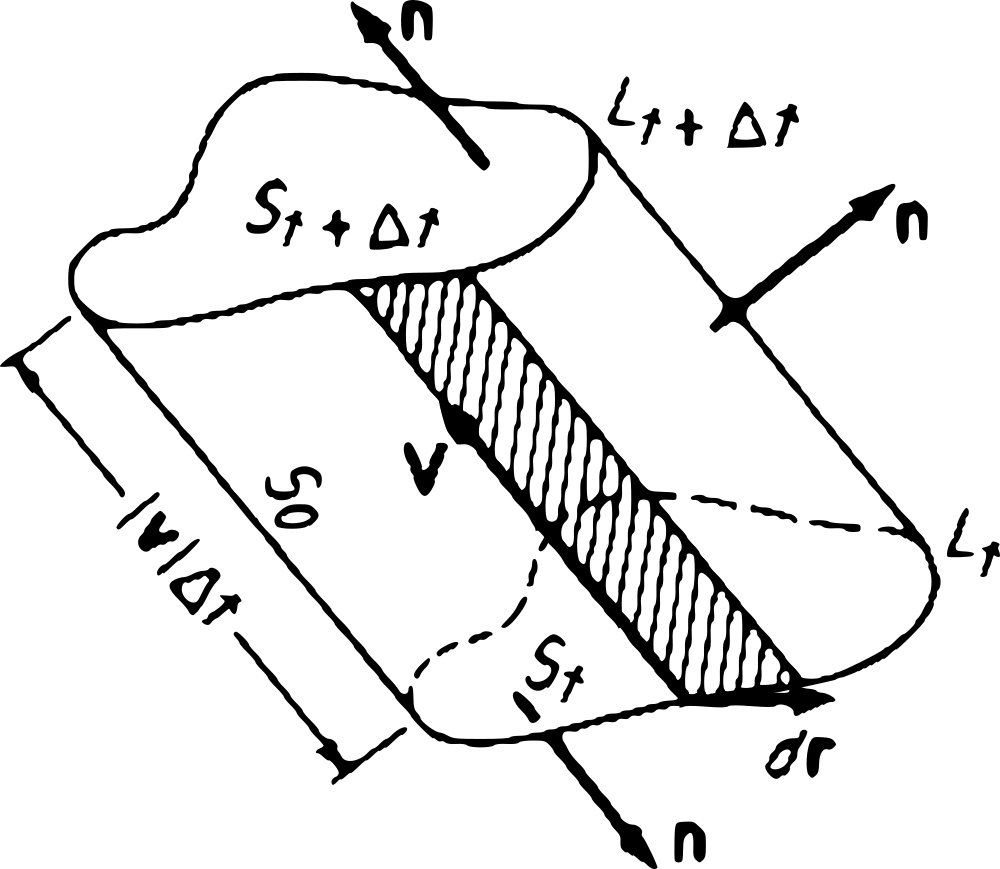
\includegraphics[width=6cm]{circulación.png}
	\label{fig:circ}
	
	\vspace{5mm}
	Figura 1
	\end{figure}		
	
	Nota: observe que el contorno $L$ también depende del tiempo.
	Pista: considere la definición original de derivada como un límite.	
	
	
\end{itemize}


\end{document}